\documentclass{report}
\usepackage[
top    = 2.75cm,
bottom = 2.50cm,
left   = 3.00cm,
right  = 2.50cm]{geometry}
\usepackage[hyphens]{url}
\usepackage{hyperref}
\usepackage{cite}
\usepackage{setspace}
\usepackage{algorithm}
\usepackage{algpseudocode}
\usepackage{graphicx}
\usepackage{rotating}
\graphicspath{ {./images/} }
\title{\vspace{-2.0cm} Automated Bayesian optimization for cloud configurations across multiple providers using a generalizable framework. \\ \vspace{0.5cm} \large Supervisors: Adam Barker \& Yuhui Lin}
\date{2019-06-06}
\author{Jack Briggs - 140011358 \\ MSc Data-Intensive Analysis}
\doublespacing
\begin{document}
\pagenumbering{roman}
\maketitle
\newpage
\chapter*{Abstract}
This study details the development of a system for automated selection of optimal cloud configurations. A generalizable framework for any searching strategy across cloud services is first designed, composed of modular components: A Searcher, for managing an optimization process; a Selector, for interpreting variables representing the encoded search space and outputting an available cloud configuration; a Deployer, for deploying the user-provided application and returning its logs; and an Interpreter, for converting these logs into an objective measure to be minimized or maximised by the optimization process. 

A use-case is presented for this framework, where a Bayesian Optimization searching strategy is used to predict the most cost-effective compute instance available across multiple providers (Google Compute Engine and Amazon EC2) for running video transcoding operations. An instantiation of the framework is implemented, capable of performing this use-case. An evaluation shows that this implementation selects optimal configurations with \textasciitilde{}90\% accuracy, a similar success rate to other more specialized solutions. Allowing 2 concurrent sampling jobs decreases search time without negatively impacting search effectiveness, but allowing further concurrency causes decreased effectiveness without further reductions in search time. Within-instance variability for performance of the use-case application was consistently below 3.23\%. AWS instances consistently outperformed Google instances at video transcoding operations, but cloud provider was the least important factor out of vCPU number and instance category in determining cost effectiveness.

The study concludes by emphasising the extensibility of the framework and system, suggesting future components for replicating previous specialized solutions, or searching serverless services and GPU instances.
\newpage
\chapter*{Declaration}
I declare that the material submitted for assessment
is my own work except where credit is explicitly
given to others by citation or acknowledgement. This
work was performed during the current academic year
except where otherwise stated.
The main text of this project report is 14,935 words
long, including project specification and plan.
In submitting this project report to the University of St
Andrews, I give permission for it to be made
available for use in accordance with the regulations of the University Library. I also give permission for the title and abstract to be published and for copies of the report to be made and supplied at cost to any bona fide library or research worker, and to be made available on the World Wide Web. I retain the copyright in this work.
\newpage
\tableofcontents
\listoffigures
\newpage
\pagenumbering{arabic}
\chapter{Introduction}
\section{Cloud Computing}
Cloud computing is an ever-growing field that now ranges from Infrastructure-as-a-service (IaaS) to Software-as-a-service (SaaS). Services under cloud computing are characterised by their ability to offer access to a shared pool of highly elastic on-demand computing resources that offer broad network access \cite{Pallis2010, Mell2011}. Cloud services as an industry has had explosive growth, and it has been predicted that 83\% of enterprise (companies with 1000+ employees) workloads will be in the cloud by 2020\cite{Intricately2019}, with 41\% of those run on public cloud platforms such as Amazon AWS and Microsoft Azure. Services offered range in various forms and levels of abstractions, from directly provisioning Virtual Machines (VMs) or storage services, allowing users full control over their cloud infrastructure, to deploying 'serverless' containers, where the actual managing of the hardware is instead handled by the cloud provider.

\paragraph{}
The appeal is obvious, with cloud services allowing organizations and developers to utilize a diverse range of computational resources on demand without any up-front commitment or cost\cite{Armbrust2009}. This can lead to significant cost-savings, as well as improved revenue through generating better customer experiences and facilitating risk-free experimentation\cite{Power2018}. Academics, too, are utilizing the services as volumes of data grow impractical to store and analyse on local machines\cite{Berriman2013, Ruiz-Alvarez2011}. This includes large-scale collaborative projects involving huge data sets hosted on the cloud such as the 1000 Genomes Project\footnote{\url{https://aws.amazon.com/1000genomes}} or Common Crawl\footnote{\url{commoncrawl.org}}.

\subsection{Cloud optimization}
This rapid expansion and uptake has led to a wide assortment of applications either being deployed on cloud services or making use of data stored on them. These applications range from one-time academic data analytics jobs mentioned to long-running media-streaming servers such as those used by Netflix or Twitch\cite{Bilal2017}. The resource dependencies of these applications also vary widely, from CPU dependent data analysis tasks to network-heavy streaming services. The performance of these applications can have very different relationships with the computational resources available from different cloud services. For example, VMs vary, both within and between cloud providers, in terms of memory amounts and the number and speed of virtual CPUs (vCPUs). While medium-length video transcoding operations benefit primarily from faster processing speeds, data analysis tasks involving large datasets may find a more cost-effective option in prioritising VMs with local solid-state drives (SSD) offering high I/O performance. Non-critical batch workloads can often benefit from using 'pre-emptible' or 'spot' instances, which offer large discounts on the condition that your machine can be terminated with little notice to free up resources. Finding out what computational resources are important to a given application, and choosing the appropriate cloud service accordingly, can be extremely difficult but can offer significant benefits.

\subsection{Benefits}
It is desirable for both users and providers to optimize purchased cloud configurations to best serve the needs of their applications. Users who fail to do, either provisioning VMs that are too powerful or too weak, risk paying far more than they need to on a given application for comparable or worse performance. A given data analysis task can cost around 3.4 times as much on an average configuration compared to the optimal available option\cite{Alipourfard2017}. Even the emergence of serverless services, in which VM allocation is almost entirely managed by the cloud providers rather than the user, simply shifts the burden of optimization from the users to the cloud providers. And for providers too, much like with load-balancing, optimizing VM allocation of user applications in cloud datacentres is important to best utilize available computational resources. Cloud datacenters in general exhibit very low resource utilization\cite{Reiss2012}. Efficient deployment to reduce unused resources across available VMs frees up extra resources for other purposes or other customers. Alternatively, identifying and avoiding the co-location of CPU-intensive workloads can reduce resource contention amongst users, leading to improved performance \cite{Pu2010}.  In addition, energy-related costs make up to 42\% of managing a data-centre, and the ability to idle inactive resources would lead to a significant reduction both in energy cost and negative environmental impact. \cite{Berl2010, Gkatzikis2013}. 

\subsection{Challenges}
Picking an optimal cloud configuration for any given application is far from trivial however. 'Larger' VM types may not provide improved performance \cite{Yadwadkar2017}, or may do so but at a far less cost-efficient rate than a cheaper 'smaller' alternative. Even if one is provided an exact budget and set of constraints placed on an application's performance, they must still find a way to search or model this performance across the entire range of services and cloud providers to ensure they have found an optimal, or at the very least acceptable, cloud configuration. This is further complicated by the variety of VM types available across multiple providers, and the variation in performance between VMs of the same specification due to differences in underlying hardware, network traffic, and co-located tenants located on the same physical machine.

\subsubsection{Search space}
The diversity in services provided by different cloud providers creates a large search space. At the time of writing, Amazon EC2\footnote{\url{https://aws.amazon.com/ec2/}} alone allows users to provision VMs from over 200 predefined 'instance' models\footnote{\url{https://www.ec2instances.info}}.dfas Google Compute Engine\footnote{\url{https://cloud.google.com/compute/}} allows users to define their own machine types, ranging from small VMs with 1 vCPU and 1 GB of RAM to 96 vCPUs with 624 GB of RAM\footnote{\url{https://cloud.google.com/custom-machine-types/}}, and includes options for specifying the CPU platform or adding GPUs. VMs can also differ in terms of network performance, local storage, CPU speed, underlying hardware, and can start up running a selection of various operating systems and associated software. 
\paragraph{}
The search space is not just challenging in terms of range, but is also hard to define in terms of constraints. Many hardware options are precluded by or only permitted alongside other options. To simplify selection, leading providers generally categorize instance types, splitting them into groupings such as 'compute-optimized' and 'memory-optimized' machines, each of which is made up of VM options of various 'sizes,' such as 'tiny,' 'small,' 'large,' referring to the amount of computational resources available to that VM. Even with this categorization, it can be hard to determine a method to formalize or encode the search space in such a way to best serve an automated optimization algorithm.

\subsubsection{Hardware and Software Heterogeneity}
Despite two VMs sharing the exact same configuration, if their underlying machines possess different physical hardware then their performance can differ significantly\cite{Leitner2014}. Amazon's M4 instance types, for example, can come with either 2.3 GHz Intel Xeon® E5-2686 v4 (Broadwell) or a 2.4 GHz Intel Xeon® E5-2676 v3 (Haswell) CPU, based on the machine they happen to be hosted by\footnote{\url{https://aws.amazon.com/ec2/instance-types/}}. However, recent studies involving recently available instance types have shown a dramatic reduction in this CPU-based variability for certain instance types\cite{Davatz2017, Laaber2019}. 
\paragraph{}
But problems regarding hardware heterogeneity expand further when searching across multiple providers. Different providers may use very different underlying CPU hardware with different clock speeds for machines reporting the same number of vCPUs. Software too, can differ. Amazon instances come preconfigured according to a template referred to as an Amazon Machine Image (AMI)\footnote{\url{https://docs.aws.amazon.com/AWSEC2/latest/UserGuide/AMIs.html}}, while Google Compute Engine instances use a predefined boot disk. These images include an operating system and associated software, storage snapshots, launch permissions, and device mappings. The APIs used to communicate with cloud providers, in order to set up cloud services, similarly differ between providers. Even when using Infrastructure as code (IaC) tools, the nomenclature and configuration file structure between providers can differ widely.
\paragraph{}
When searching across multiple instance types, the hardware and software heterogeneity must be taken into account, especially when the search spans separate cloud providers. 
\subsubsection{Variation}
Even when run on identical cloud configurations from the same provider, the same application or benchmark can have significantly different performance, more so than is observed when run in on-premise environments\cite{Leitner2014}. This is in part due to hardware heterogeneity in underlying machines as described above, but can also occur due to multitenancy, where multiple customers may share computational resources by running VMs on the same physical machine. This can lead to a slowdown in one instance due to the behaviour of another colocated tenant. This problem is referred to as the 'noisy neighbour' problem\cite{Gkatzikis2013}. Disk I/O operations or network traffic between instances and storage disks could similarly be affected by the machines' relative locations within or between datacentres. 
\paragraph{}
All the above problems causing variation within instance types are generally out of the control of the customer. Cloud providers may be developing methods of minimising the problems, shown by the recent reduction in the variation of intra-cloud network performance\cite{Scheuner2018, Scheuner2018a} and CPU performance between identical instance types \cite{Davatz2017, Laaber2019, Scheuner2018}.  Nonetheless, in cloud configurations where this variation is still significant, it add a significant element of randomness to the performance of various applications on cloud services. This randomness must be accounted for by any method used to optimize cloud configurations, and rules out assumptions of deterministic application performance. 
\subsubsection{Application range}
As mentioned earlier, numerous types of applications are deployed on the cloud, from long-running web-servers and media-streaming services to one-time data analytics jobs. The performance and cost-effectiveness of these applications can have very different non-linear relationships with cloud configurations, making them difficult to model analytically, even if the contents of the application are known exactly. In some cases, such as in serverless container services like Google Cloud Run\footnote{\url{https://cloud.google.com/run/}}, the application is not known at all, and must be treated as a black box. \\
To ensure an optimization method is as generalizable as possible, it must be able to utilize user's specifications and the outputs of an application, but must treat the application itself as a black box, and not make hard assumptions regarding any of its characteristics or its relationships with configuration options.
\subsubsection{Objective measure}
Finally, the very meaning of the word optimal can depend on the application and the user. The ultimate goal is far from fixed. For a server, optimizing for a good mean performance may fail to optimize for high workload situations, leading to lower-than expected performance under these conditions. Even in single batch jobs, different users may tolerate different reductions in performance for different cost-savings. While an effective option is to simply present to the user an informative representation of how cost and performance vary with cloud configuration options, allowing them to decide on their own trade-offs between cost and performance, this is not possible in many black-box options and limits the level of automation in the optimization process.\\
To truly automate an optimization process for any provided application, an 'objective measure' must be provided, dependent on cost and performance, which reflects the ultimate goal of the optimization process. It might be a job's runtime divided by the price of a configuration, to be maximised, or a server's maximum latency given a specified workload, to be minimized. An optimization method must be able to accommodate different user requirements, allowing flexibility based on the the objective measure used.

\section{Aims and Objectives}
The primary aim of this project is to present a fully automated system to search for an optimal cloud configuration across multiple cloud providers for any given application. The system should, as best as possible, overcome the challenges we have presented in the above section, while being as generalisable as possible for any forms of application or cloud services. To make the system generic and allow for any cloud-based optimization search strategy, such as Bayesian optimization or grid search, a generalizable framework should be first designed.

We hope to to deliver an instantiation of the framework, using Bayesian optimization for multiple cloud providers. As a motivation, we will present an example use-case, relevant to modern cloud applications, composed of an application, objective measure, and search space. We will implement the instantiation as a fully functioning system that can, at a minimum, carry out the optimization search this example use-case entails.

Once this system is implemented, we will use it to evaluate our framework and system, as well as gather data to analyse the state of cloud variability and relative performance measures across different cloud services for our use-case application.  

To achieve these aims, we must succeed at the following objectives:
\begin{itemize}
\item Design a framework for fully automated and generalizable optimization of a cloud configuration for a given application.
\item Present an example use-case of an application and set of cloud services for which an optimal cloud configuration is to be found.
\item Develop a fully functional system of our framework that is, at a minimum, capable of carrying out a search to find the optimal cloud configuration for the example use-case
\item Evaluate our framework and system, determining effectiveness and relationships to different settings, uses, and options.
\item Analyse results to describe the current state of cloud variability and relative performance predictions between the cloud services examined.
\end{itemize}

% ALTERNATIVE AIMS AND OBJECTIVES:
%The aim of this project is both to present a framework for completely automated selection of an optimal cloud configuration for any given application, as well as to deliver a fully functional implementation of this framework for an indicative use-case. To achieve this aim, the framework must achieve the following objectives:
%\begin{itemize}
%\item Present a fully automated process for optimizing a cloud configuration.
%\item Be applicable for any form of cloud application.
%\item Not be limited to any one cloud provider or service.
%\item Take into account variation within and between instance types.
%\end{itemize}
%
%In addition, we wish to deliver a fully functional implementation for an indicative use case, which will achieve the following objectives:
%\begin{itemize}
%\item Automate selection of cloud configuration samples based on a search space of cloud configurations spanning multiple providers.
%\item Provision specified instance types from multiple providers based on a given cloud configuration.
%\item Deploy and return logs for a given application on a given cloud service based on a given cloud configuration.
%\item Interpret logs based on the performance and cost of a given application on a given cloud configuration.
%\end{itemize}

\section{Contributions}
For this project we designed a generalizable automated cloud configuration selection framework, implemented an system of that framework for a Bayesian optimization use-case, and analysed the results to look at trends in cloud performance, its variability, and how job concurrency or number of cloud providers can affect a Bayesian Optimization search.

Some highlighted contributions are:
\begin{itemize}
\item We present a framework for fully automated selection of the optimal cloud configuration for any search space, type of application, or optimization algorithm.
\item We present and have made publicly available an system for a Bayesian Optimization search to find the most cost-effective machine available on Amazon EC2 or Google Compute Engine for a video transcoding task. The source code of the system is available at: \url{https://www.github.com/briggsby/AutomatedBayesCloudSelection}
\item The above system consists of modular components that can easily be switched out depending on use-case, and we show how this can be done.
\item We show that variability in performance between instances of the same type has dramatically decreased in recent years.
\item We show that, at the time of writing, Amazon EC2 instances consistently outperform Google Compute Engine instances at video transcoding tasks.
\item We show that Bayesian Optimization does not reduce in effectiveness when the search space is expanded to include multiple providers, at least when there is a clear performance difference between them.
\item We show that allowing additional concurrent sampling jobs for a Bayesian optimization search was beneficial at first, but allowing too many (3 in our case) reduced search accuracy.
\end{itemize}
 
\section{Dissertation Outline}
This report consists of 9 chapters, which together identify and explain the problem of cloud configuration selection, eventually describing the development and evaluation of a tool to enable generalized automated selection of the optimal cloud configuration for an application.

\paragraph{Chapter 1 (Introduction):} Describes the background of selecting optimal cloud configurations, and identifies the importance of and challenges with developing an automated and generalizable tool to do so. Also presents our overall contributions and this outline of our submitted report.
\paragraph{Chapter 2 (Literature Survey):} Surveys the literature surrounding cloud configuration selection. The chapter discusses previous studies examining cloud performance variability, automated configuration selection, and the use of benchmarks to evaluate cloud performance.
\paragraph{Chapter 3 (Requirement Specifications):} We present an example use-case of an application that needs an optimal cloud configuration found within a specified search space, and use this to define the requirements that our framework and system must achieve to be considered successful.
\paragraph{Chapter 4 (Generic Automated Cloud Configuration Optimization Framework):} We present the full design of our generalizable framework, as well as the motivations behind those decisions.
\paragraph{Chapter 5 (Bayesian VM Optimization System):} We present the additional design considerations for our specific implementation of the framework described in Chapter 4, guided by our example use-case described in Chapter 3.
\paragraph{Chapter 6 (Implementation):} Implementation notes for our developed system for the example use-case described in Chapter 3, explaining use of associated tools or libraries and describing modifications or changes made to them.
\paragraph{Chapter 7 (Evaluation):} We evaluate our framework and system against the project goals, as well as analyse results from our experiments to look at how searches and performance are affected by search settings or cloud configuration options.
\paragraph{Chapter 9 (Conclusion):} We conclude by critically discussing our project as a whole, and comparing it against other related work. We examine the impact of our contributions and discuss directions for further research.

\chapter{Literature Survey}
\section{Cloud services}
% CAN WE GET A STUDY TO JUSTIFY FOCUSING ON COMPUTE SERVICES? SHOWING THAT THEY'RE THE PREDOMINANT FORM?
There is now a huge array of cloud services available, specialized for different forms of applications or use-cases. Dozens of cloud providers offer a variety of different services, billing options, support, and resources\footnote{\url{https://www.cloudorado.com/cloud_providers_comparison.jsp}}. Going into detail on every service offered would be a vast, if impossible, task. We primarily focus on 'compute' services, which provide Infrastructure as a service (IaaS) in the form of VMs to run applications such as data analysis jobs or web-severs. AWS alone offers many different compute services, ranging from Amazon EC2 where the user can specify individual VMs in the form of 'instances' of various types each with their own set computational resources, to AWS Fargate\footnote{\url{https://aws.amazon.com/fargate/}}, a 'serverless' option where users provide containerized applications to be run and the provider manages any hardware management, load balancing, and administration. Most of these services have analogues on other providers, such as Google Compute Engine for Amazon EC2 or Google Cloud Run\footnote{\url{https://cloud.google.com/run/}, beta at the time of writing} for AWS Fargate. Once a service is selected, along with the chosen cloud provider, there is usually a number of configuration options available for users. For example, even for AWS Fargate users must specify the CPU and memory requirements of their application. For Amazon EC2, as described in the previous section, there are over 200 instance type options to choose from, depending on region, each with their own computational resource specifications.

As well as creating a huge search space for any optimization task, the differences in terminology or API specifications between providers complicate automated tasks. To help manage this, various tools described as 'Infrastructure-as-code' (IAC) have been developed which provides higher-level abstractions for many of the specifications that must be provided when utilizing IaaS-based cloud services. 

As mentioned in the previous chapter, another hurdle is the variability in performance for applications hosted on cloud services. Even performance for the same application on the same instance type can vary more than is observed for on-premise environments \cite{Leitner2014}. Here, we look at the literature examining the variation and see how it has decreased over time, and determine if it is still an important factor in a search for an optimal configuration.

\subsection{Cloud variability}
An extensive review of cloud variability showed that in 2014, cloud performance variability was quite significant and relative standard deviations for performance metrics for cloud VMs were generally above 5\%, depending on providers and instance types\cite{Leitner2014}. For I/O-based tasks on some Microsoft Azure\footnote{\url{https://azure.microsoft.com/}} or AWS VMs especially, huge variation in tasks meant that performance on one VM could be almost double that of another VM of the same instance type. For CPU-based tasks, the variability could range from almost negligible to over 20\%, though it usually dropped to extremely small values when differences in underlying hardware were taken into account. Network performance too varied considerably, enough to, along with the other hardware-dependent variations, encourage 'placement gaming' strategies to actively exploit performance heterogeneity to lower costs\cite{Farley2012}.

\paragraph{}
Some time has passed since these studies, however, and newer instance types are now available. On AWS, for example, these studies mostly looked at 1st to 3rd generation instance types, while 5th generation instances are now available. The 3rd generation AWS instance types looked at in \cite{Leitner2014} had considerably less variable performance than those from the 1st generation.

In 2018, a study into a cloud benchmarking suite found that intra-cloud network performance had achieved 'almost perfect stability'\cite{Scheuner2018, Scheuner2018a}. CPU performance, too, had become predictable with less than 0.3\% relative standard deviation\cite{Scheuner2018}. I/O variability could also be drastically reduced by switching from HDD to SSD disks. Several benchmarks already reported much more stable performance measures using newer cloud instances, often below 5\%\cite{Davatz2017, Laaber2019} These reductions in variability have reduced the incentive for placement gaming approaches, and may serve to reduce or even eliminate the impact sampling noise has on performance measurements of cloud configurations. However, how much variability still remains seems hard to predict for a given application without directly examining the variability of that application's performance provided by a given configuration.

\section{Previous Work}
Many previous studies have addressed the issue of cloud configuration optimization, presenting possible solutions. However, these solutions are usually limited in scope, such as to single providers or specific application types. In addition, they have rarely, if ever, provided an available associated instantiation of their system, capable of carrying out the processes they design and evaluate. In this section, we look in detail and compare previous notable solutions to the problem.

The cloud optimization systems previously performed generally utilize one or more of the following important methods: modelling, sampling, and benchmarking. 

\paragraph{}
Modelling methods try to analytically estimate relationships an application type will have with the computational resources provided by different instance types. If not performed together with sampling, this requires at least a cursory understanding of the application itself, such as its bounding resource or disk capacity requirements, but can provide an estimate extremely rapidly. Modelling methods can range from simple decision-trees or flowcharts, followed by an automated system or human, to complex predictions of large data analysis jobs based on the same job's performance on smaller datasets. This latter method is performed by Ernest\cite{Venkataraman2016}, the first solution we examine below.

\paragraph{}
Sampling methods take multiple performance samples from the available range of cloud configurations. These samples can then be used to either approximate an effective option by returning the best-tested configuration, or to generate a model for how that application's performance will change based on configuration options. An example of a method that uses only sampling is an exhaustive search, a brute-force method that samples every available cloud configuration, possibly multiple times, to return with utter confidence the optimal cloud configuration. Alternatively, sampling can be used together with modelling or benchmarking to predict application performance on some configurations indirectly, reducing the number of samples necessary.
In a non-recurring batch job, sampling the exact job itself is counter-productive, as it would require the job to be run multiple times just to find out which machine would have done it best. However, for batch jobs the cost of the initial performance testing can be offset by later repeats. In 2012, it was reported that up to 40\% of Microsoft's analytics jobs are recurring \cite{Agarwal2012,Ferguson2012b}. Sampling has the benefit of not requiring any prior understanding of the application itself, an essential quality in our aim of generalizability, but has the drawback of requiring costly sampling from the cloud configuration. Most of the previous solutions examined in this section use some searching.

\paragraph{}
Finally, benchmarking methods may indirectly approximate the performance of an application by instead using indicative benchmarks or micro-benchmarks. When used with sampling, benchmarks can dramatically reduce the cost of sampling, as they are generally cheaper to perform. They can even eliminate the cost, as a benchmark run once can be later used to predict the performance of several applications with a known relationship with it. However, benchmarking can sometimes be a poor indicator of performance for an actual application, and use of it at all still requires some understanding of how that benchmark relates to the applications performance. We describe the state of cloud benchmarking in more detail in the next section.

\subsection{Ernest}
Ernest\cite{Venkataraman2016} is a framework that aims to predict the performance of given data analytics jobs by generating a performance model based on the job's performance using different samples of the provided input data. These performance samples using smaller datasets typically take much less time and resources to run than the full job, reducing the overhead for finding an optimal instance type for the full job. For generating the model, Ernest relies on the assumption that there is a relatively simple relationships between computational resources and the job performance, allowing it to  produce the model by estimating a few pre-set linear terms. This assumption generally holds when it comes to big data analytics jobs, as the size of the jobs have encouraged algorithms that scale well in a linear or quasi-linear manner\cite{Bottou2008}. In cases where more complex models are needed, small extensions can be used to adapt the model to the use-case. In their evaluation, it is shown that Ernest provides predictions for job performance with ~15\% error with a training time ~4\% of the total job runtime.

% GET A CITATION FOR THE 'UNLIKELY THAT' BIT
While Ernest is an effective method for reducing search cost and time without impacting predictive capabilities, it is very specific for data analytics jobs. For many applications, it is unlikely that performance can be modelled in terms of computational resources through pre-set simple linear or quasi-linear terms. It also does not cover the task of provisioning the instances from cloud providers, but rather requires instances to be already set up running an Apache Spark cluster. No associated publicly available instantiation of their system is provided.

\subsection{CherryPick}
CherryPick \cite{Alipourfard2017} is similar to Ernest in that it uses samples from the search space to model relationships between the performance and computational resources for a given batch job. However, CherryPick does so using Bayesian Optimization, a very generalizable optimization process that models the relationships as Gaussian processes without making assumptions as to linearity or monotonicity. Bayesian optimization has the added benefits of incorporating sampling noise and being designed to minimize the number of samples necessary. Despite reducing samples through this method, CherryPick assumes that the full job must be used for samples, and so is only beneficial for recurring jobs. CherryPick was directly compared to Ernest, and for that comparison was found to produce much better estimates, though it did so with 11 times the search time and 3.8 times the search cost\cite{Alipourfard2017}. 

Along with PARIS, CherryPick presents the most promising solution we detail here for a truly generalized method, through its use of Bayesian Optimization. It includes in its design a 'Cloud controller' component to provide the VM provisioning process, as well as a 'Cloud monitor' to monitor performance noise in the cloud for use by the Bayesian optimization engine. However, in the framework described it is limited to recurring batch jobs, as it bases its decisions entirely on the time taken to perform the submitted job and the cost of the configuration used. In addition, the paper details very little about the design and implementation of these Cloud components, and no publicly available instantiation of the framework is provided.

\subsection{PARIS}
PARIS \cite{Yadwadkar2017} presents an ingenuitive method of predicting performance by using random forests to model how an application's performance relates to a benchmark's performance, rather than to cloud configuration variables directly. It can then compare this to historical benchmark data to predict performance on different cloud configurations. For instance types hosted on AWS, this allowed predictions with $<$20\% error using only samples from a few reference VMs.

PARIS is an extremely promising solution, offering both generalizability and very low overhead by levering historical benchmark performances, along with various other performance metrics collected during these benchmarks. While generating this initial benchmark data is expensive, in terms of cost and time, it can be reused for many different applications, depending on the breadth of the benchmarks. That said, the solution is dependent on ow well their performance can be modelled to the performance of the tested application. Once again, no associated publicly available instantiation of the system is provided, and the framework does not include any details on VM provisioning or communication with the cloud provider.

\subsection{Smart Hill-Climbing}
Smart Hill-Cimbing for finding optimal configurations for web-server based applications was introduced back in 2004\cite{Xi2004}, without any mention of cloud computing (AWS was released in 2006\footnote{\url{https://aws.amazon.com/about-aws/whats-new/2006/08/24/announcing-amazon-elastic-compute-cloud-amazon-ec2---beta/}} or any form of IaaS. It modelled a web-server based application as a black box function with an output of some metric to be minimized or maximised such as throughput, response time, or a value related to multiple other metrics. In Smart Hill-climbing, a weighted form of Latin Hypercube Sampling\cite{McKay2000} is used together with modelling small locally bound relationships between the function's output and its variables as quadratic terms to rapidly sample across the entire search space searching for a global minimum.

While an old paper, with no notes on implementation with regards to cloud-based deployments, the paper presents an effective method of modelling an application, for example a web server, as an objective function for a generalized optimization algorithm. Smart Hill-Climbing makes use of repeated Latin Hypercube Sampling to avoid falling into local minima, and makes use of locally bounded quadratic function models to guide the search without making specific assumptions about the objective function. Like Bayesian optimization, it is effective for optimizing expensive functions due to the low number of samples required to make confident predictions. 

\subsection{Others}
% ADD IN SHORT SENTENCE TO SAY SHORTCOMING OF DALEEL, AND MAYBE FOR ELASTICIZER
To briefly mention other related works; Elastisizer\cite{Herodotou2011} uses previously generated profiles and recursive random searches to model the performance of MapReduce tasks on cloud clusters. Daleel\cite{Samreen} presents a framework for collecting and utilizing data for generating machine-learning-based models to predict application performance on cloud configurations. \cite{Bodik2009} uses non-linear regression models and to find the cheapest configuration that satisfies user-provided Service Level Agreements (SLA) for a horizontally-scaled webserver. \cite{Bodik2009} does this by exploring configurations through increasing or decreasing the number of instances in a cluster according to whether a latency threshold set by the SLA is being breached or met. 

\section{Benchmarking}
Benchmarking in the cloud is the process of evaluating a service or VM by comparing its average performance at a certain task against a standard reference\cite{Binnig2009}. For example, you may see how many times a VM can calculate the number of prime numbers below 10,000 in ten seconds. This specific example would be an example of micro-benchmarking, where rather than evaluating performance for a complex task such as video transcoding, you are using a very quick (e.g. $<$1 ms) repeated task that isolates and evaluates one specific 'software unit,'\cite{Laaber2019} in this case a prime-number counting method to benchmark specifically the CPU speed of the VM.

A good benchmark for cloud computing is one that, for your specific application, allows you to accurately, as well as quickly and therefore cheaply, estimate the performance a service or VM would provide on your application. This is useful when the application itself is either costly to run to completion or can perform several different workloads each of which has a performance that can be estimated from benchmarks.
In addition, cloud computing presents its own challenges for benchmarking. The increased variability in performance can cause estimates to be less accurate, and the benchmarks themselves should have an automated deployment method such as a Docker container. In addition, performances are mostly only relevant relative to the price of the services that offer them\cite{Binnig2009}.

\chapter{Requirements specification}
\section{Use-case}
Here we present a specific use-case with which to implement and evaluate our eventual framework. This use-case should be relatively general while still providing a good example to directly evaluate the effectiveness of our framework. To this end we have chosen the following use-case: Performing a Bayesian Optimization search to predict the most cost-effective instance type for a vBench benchmark score, out of instance types available without quotas on Amazon EC2 and Google Compute engine.
\subsection{Search space}
We chose the search space to best enable replication in the future by ensuring that all instances were available without requesting additional quotas from the cloud providers, as well as being relatively cheap options so as to reduce search costs. We wanted to ensure that our search could span multiple cloud providers, and so we chose two leading providers who had equivalent instance types that fit the above criteria. We opted not to go for a serverless option due to the lack of an Infrastructure-as-code implementation for Google Cloud Run and to increase the number of available variables that would have to be optimized by a search.
\subsection{Bayesian Optimization}
We chose Bayesian Optimization as it seemed like one of the more generalizable and effective solutions\cite{Alipourfard2017}, and was considerably less complex or costly to implement than others such as the PARIS design, which would require extensive costly benchmarking before any evaluation\cite{Yadwadkar2017}. We were confident Bayesian Optimization would function for any application for which we could extract or return a single objective measure to minimize or maximize, with relatively few samples necessary. We will use the findings from the CherryPick paper, such as effective stopping conditions, to inform our design and implementation, but will attempt to expand on their findings to see how Bayesian optimization is affected by search spaces spanning multiple cloud providers and by allowing multiple concurrent jobs.
\subsection{Video transcoding}
Video streaming is one of the most common services for which cloud servers are used, where video files are transcoded to an appropriate file type and streamed to an end-user's device\cite{JunXin2005a, Lottarini2018}.
The deployment to be used was originally planned to be Cloudsuite3's media streaming benchmark\cite{Palit2016}, however this was found to be dependent entirely on network bandwidth, and extremely variable. Instead, the vBench video transcoding benchmark was used\cite{Lottarini2018}. We will use this benchmark to measure a single instance type's relative rate of transcoding a single 5 second 1920x1080 video file of the inside of a house.
\section{Requirements}
\subsection{Framework requirements}
The framework should enable:
\begin{itemize}
\item Fully automated deployment of a given black-box application on given cloud configurations across multiple providers
\item Optimization algorithms to select and request sampling jobs which will carry out the above deployment
\item Extraction of relative performance measures and costs from sampling jobs
\end{itemize}
The framework should require only the following inputs, from which it should output a single prediction for the optimal cloud configuration:
\begin{itemize}
\item The application itself, to be set up on a given cloud service.
\item Details of the search space and its constraints.
\item An objective measure with with to evaluate cloud configurations.
\end{itemize}

\subsection{Use-case system requirements}
The system should include:
\begin{itemize}
\item A Bayesian Optimization engine that searches variables representing an encoded search space of cloud configurations across multiple providers
\item Configurations for an IaC tool, which provision a specified cloud configuration from a given provider, that cover the entire provided search space
\item A deployment method to run the provided vBench benchmark on the provisioned VMs and return performance scores
\item The ability for the Bayesian Optimization engine to request multiple sampling jobs at a time from the IaC tool and deployment method
\item Return a prediction from Bayesian Optimization for the cloud configuration with the best performance/cost ratio. The error in this prediction should be relatively low, accommodating the flexibility to allow reduced predictive power in return for substantially reduced search cost/time
\end{itemize}

\chapter{Generic Automated Cloud Configuration Optimization Framework}
\section{Design Motivations}
\subsection{Numerical Optimization}
In any optimization process, the value of some objective function is minimised or maximised by adjusting its input variables or parameters. An optimisation algorithm begins with an initial guess of these variables and iterates through improved estimates until they terminate, hopefully providing an estimated solution \cite{Nocedal2006}. An optimization function effectively takes as inputs an objective function, along with its previous inputs and outputs, and outputs either the next sample to take, or the predicted best input if the stopping condition is met. \\
In our generalized case, the optimisation method and objective function are both unknown, but we know that our objective function will always involve selecting some cloud configuration based on the inputs that describe that configuration, deploying some application onto this configuration, and interpreting its performance to give some objective measure.
 

\subsection{Modularity}
In our generalized case, we do not yet know the optimization method or objective function. As shown in our Literature review, a number of optimization algorithms have been attempted and are available, such as exhaustive search, Bayesian optimization\cite{Alipourfard2017}, analytical methods that directly model the application's relationships with configuration variables\cite{Venkataraman2016}, and a data-driven approach predicting performance by its relationship with pre-run benchmarks\cite{Yadwadkar2017}.

Much like how our objective measure will differ from application to application, the best optimization method may also differ depending on the type of application tested. Applications whose performance is accurately reflected by known benchmarks may benefit from PARIS's data-driven approach, while situations with a large number of local minima or maxima may benefit from Smart Hill-Climbing. Because of this, it is desirable to ensure that any optimization method can be replaced by another if the user deems it more appropriate to their use-case.

Because of this, we are left with multiple parts of our system which are highly dependent on a user's individual use-case, namely the objective function, the objective measure to be optimized, the search space constraints, and the application itself. Because of this, we have taken a highly modular approach to our design. While our system should be self-sufficient to run its example case, it should also be made up of several replaceable components for future extensions. The framework itself should be well suited to any case, where for each individual component the user can use the specific implementation that is best suited for their use-case.
 
\section{System Architecture}
Our optimization process can be broken down into four replaceable components: A Searcher, which runs the optimisation algorithm, testing out various inputs in an attempt to maximise or minimise the objective function; a Selector, which interprets the inputs to determine what cloud configuration is being tested; a Deployer, which provisions the machines needed for that cloud configuration, deploys the application, and once it has terminated returns any required logs from it; and an Interpreter, which takes these logs to calculate the objective measure which is returned to the Searcher as the returned value for the objective function. A diagram of this breakdown is shown in figure \ref{fig:design}. The components themselves are examined in further detail in the following sections.
\begin{figure}[!hb]
  \centering
   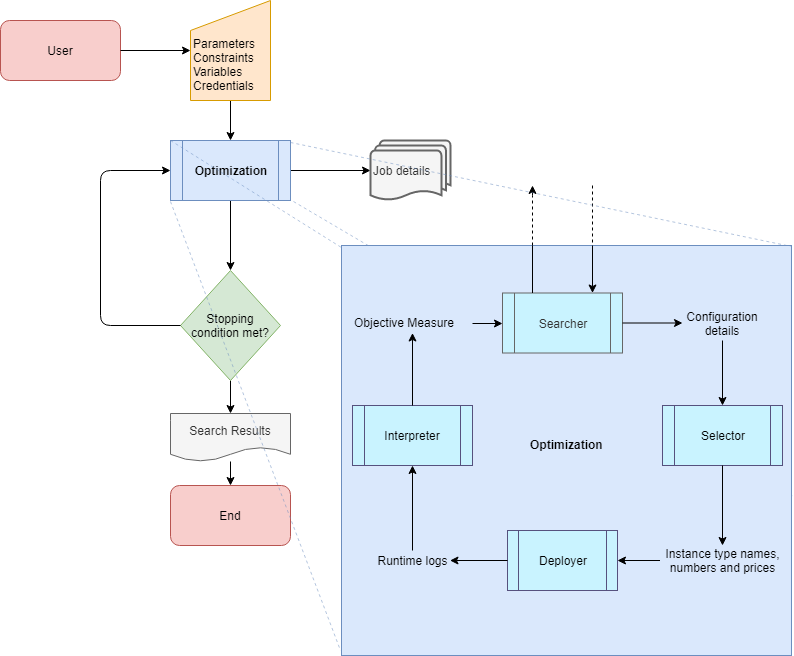
\includegraphics[scale=0.5]{Design_flowchart}
  \caption{A flowchart showing the processes involved in and information flow through the designed system.}
  \label{fig:design}
\end{figure}
\newpage
 
\paragraph{}
Overall, the system drives forward an optimization algorithm shown in Algorithm \ref{alg:Optimization}, such as Bayesian optimization, coordinate descent, Smart Hill-Climbing, or exhaustive search, by iterating through potential input variables. For each set of inputs, it take a sample from a single 'job,' where it runs through a single loop of the Selector, Deployer, and Interpreter components. The Searcher component then uses the results from inputs tried so far to choose the next set of input variables to sample, as well as provide the current estimate of the best possible set of input variables to minimize or maximize that result. Once the stopping conditions are met, the latest estimate for the best input variables is output by the system.

\begin{algorithm}
\caption{Optimization Procedure}
\label{alg:Optimization}
\begin{algorithmic}
\Procedure{Optimization}{$Starting \ variables, Stopping \ conditions, Searcher, Selector, \newline
\hspace*{4.3cm} Deployer, Interpreter$}
\State $\vec{x}_{0}\gets Starting \ variables$
\For{$i = 0,1,2,3,...$}
\State $Config_i, Price_i\gets Selector(x_i)$
\State $logs_i \gets Deployer(x_i, Config_i)$
\State $results_i \gets Interpreter(x_i, logs_i, Price_i)$
\State $\vec{x}_{i+1}, stop, best\vec{x} \gets Searcher((x_-, x_1,...x_i), (results_0, results_1,...results_i),\newline
\hspace*{5.6cm}Stopping\ conditions)$
\If{$stop$} 
\State \Return $best\vec{x}$
\EndIf
\EndFor
\EndProcedure
\end{algorithmic}
\end{algorithm}
 

\paragraph{}
It is assumed that in the vast majority of cases, the user would provide their own Interpreter and Selector. Interpreters and Selectors are very dependent on the form the application logs and search space will take respectively, and are extremely hard to generalise. For this reason, the modular design of our solution should make it simple for any component to be replaced, such as by one supplied by the user.  \\
While Interpreters and Selectors are highly specific, in only some cases should the user need to provide their own Deployer. Applications can often be contained within Docker containers, complete with requirements and runtime instructions. Because of this, aside from occasional setup such as in multi-node clusters or multi-container applications, a Deployer which provisions a given configuration from a given provider, and then deploys and attaches to a user-provided docker image to collect its logs will be sufficient.  \\
Only in rare cases would the user be required to provide their own Searcher. This is because optimization algorithms themselves should be applicable to any deployment. While, as mentioned, in some cases different searchers may be more effective, Bayesian Optimization is a good general method for predicting an application's optimal cloud configuration with reasonable accuracy with very few samples. A Bayesian Optimization implementation will be provided.


\section{Inputs and outputs}
The user inputs are shown in figure \ref{fig:design} as being made up of 4 parts: Parameters, constraints, variables, and credentials. The parameters would be options for the searching method itself, such as the stopping conditions or maximum number of concurrent jobs. Variables and constraints together define the possible search space for the input variables, as well as their starting values. Each variable must be given a type, such as string or integer, and a set of constraints such as maximum or minimum for numeric variables or the available options for categorical variables such as strings. Finally, the user would have to submit paths to the files holding the credentials to allow the program to provision and access virtual machines on the tested cloud providers. It is of course essential that credentials are never stored in any form by the program itself, and only paths to the relevant files are passed to the relevant tools and interfaces.
\paragraph{}
The figure also shows the relevant outputs created by the system in the form of 'job details' and 'search results.' These are files containing details describing the jobs performed and their individual results, as well as the final prediction for the optimal configuration produced by the system. Keeping outputs from individual jobs is important, both for debugging the system during development or component switch-over, as well as to allow users to avoid repeating unnecessary repeats of already tested configurations when performing multiple search experiments.
\paragraph{}
Algorithm \ref{alg:Optimization} shows the general form the optimization process takes with only one concurrent job allowed at any time, showing the expected input and output of each individual component. These are explained in more detail within each component's individual section below.

\section{Searcher}
The Searcher component is responsible for handling the optimization algorithm itself. It takes the results from previous jobs and determines either the next best sample to take within the available search space, or to terminate the process and return the current best prediction for the optimal configuration. 

A perfect Searcher is one that returns a perfect prediction of the optimal configuration in as few samples as possible. Fewer samples means a reduction in the time and cost taken to perform the search. Often, there is a trade-off here, where extending a search to include more and more samples, such as by setting less restrictive stopping conditions, increases its cost but also increases its predictive accuracy.

\paragraph{}
As an example, in an exhaustive search every possible combination of the inputs is sampled, giving a complete analysis of the entire search space. This obviously takes many samples, $n * \prod_{i=1}^{j} x_{i}$ where $x_{i}$ is the number of options for the \textit{i}th of J variables, and n is the number of samples taken from each configuration. This results in a large or even infinite search cost and time, but is almost certain to return the optimal result, depending on the amount of randomness involved in sampling.

\paragraph{}
Unless a job is repeated on an extremely regular basis, a user may desire to give up a small degree of accuracy or generalizability for a dramatically reduced search cost or search time. Some search methods, such as PARIS\cite{Yadwadkar2017}, can leverage past search experiments to reduce the number of samples taken. Generally however, the stopping conditions and search method will control this trade-off, and can be set according to the user's search budget or time constraints. 

\paragraph{}
In order to accurately predict the best next sample to take, the Searcher must know the available search space.  A description of how to encode cloud configurations into a set of variables and constraints is done in the Selector section. Ideally, we want our searcher to be capable of performing multiple jobs concurrently.

\section{Selector}
The Selector converts the variables provided by the Searcher component into the form of an available cloud configuration. Cloud configurations have a number of variables that can describe them, such as vCPU number, memory amount, disk speed, number of instances, instance category, machine type, and cloud provider. The selector must use whatever combination of these is provided and find either the exact or most similar cloud configuration available, passing this information on to the Deployer. In the tools used for our implementation of our system, no cross-provider API was available to directly translate machine specifications into the virtual machine types available from different providers; the Selector component bridges that gap.

\subsection{Exact vs. Closest Match}
For finding an exact match, the Selector can simply lookup the appropriate instance type from a dataset according to the input variables stored as each instance type's attributes. Looking for a closest match rather than an exact one gives more flexibility in how the input variables can be encoded, but means more complicated decisions such as attribute priority must be made, and extra assurances included to not repeat unnecessary samples when multiple sets of inputs describe the same closest input type. For our use-case, we will specifically use the simpler Exact Match method, but thanks to the modular design it will be easy to extend to include a Closest Match Selector option if time allows.


\section{Deployer}
The Deployer deploys the user-provided application, batch job, or benchmark onto the selected cloud configuration, and collect any necessary analysis from it. Typically this will involve provisioning the necessary machines from the given provider, followed by deploying the given application onto these machines, and either collecting logs from them or from a networked instance or cluster. 

\subsection{VM Provision}
Aside from in serverless computing, a necessary step of deploying any cloud-based application is provisioning the VMs themselves from a cloud provider. The Deployer should be capable of requesting any set of VMs chosen by the Selector, regardless of provider. This can be simplified using Infrastructure as code (IaC) tools such as Terraform, which offers the ability to codify the APIs from many different providers into declarative configuration files. As long as configuration files and credentials for use by an IaC tool are supplied for each possible provider, then a Deployer can call the IaC tool and corresponding configuration to provision the machines. 

There are several requirements for an IaC tool that is used for this. As instance type and number of machines will be supplied by the Selector, and therefore cannot be known until the machines are provisioned, either these details must be declarable as variables when the tool is run, or the configuration files must be suitable for automated editing just beforehand. Along with this, the tool must support multiple concurrent tasks with their own specifications and outputs, if we hope to allow the Searcher to take multiple samples at once.

\subsection{Application Deployment}
Once the VMs themselves are provisioned, the application must be set up on them and run. There are many forms this application can take. For our use-case, we have assumed the application is fully contained within a single Docker image. This enables effective deployment both on single machines as well as by cluster-based container-orchestration systems such as Kubernetes. Pre-built Kubernetes clusters are offered by several leading cloud providers. 

That said, other types of applications not fully contained within a single image are common, such as micro-service based web applications. Alternatively, an application's performance might be poorly estimated internally, and best estimated by its response over a network. Once again, the modular design allows users to implement their own Deployers to deal with alternative situations.

\subsection{Simulated Deployment}
It may be advantageous, especially during debugging or if using a 'closest match' approach to configuration selection, to instead either simulate the response from provisioning and deployment of an application, or to return a previously sampled response. It is therefore useful to ensure full logs of any deployment are stored so that, if desired, future calls to 'Deploy' an already sampled configuration for a given application can simply be responded with a value based on previous results from the same configuration.

\section{Interpreter}
The Interpreter must interpret whatever logs or other information is returned by the Deployer, along with the cost of the cloud configuration provided by the Selector, in order to return an objective measure for the sampled cloud configuration. It is this returned value that the Searcher will be attempting to minimise or maximize. We leave it to the user to develop an Interpreter for their use-case. This will likely involve extracting relevant information from the deployed application's logs, and applying constraints based on the time taken or machine pricing. 

\chapter{Bayesian VM Optimization System}
In this chapter we describe the design considerations for the example use-case system, which will operate within the framework presented in the previous chapter.

\section{Bayesian Optimization}
Bayesian Optimization is an optimization method specifically designed for situations where the objective functions itself is unknown beforehand and expensive to perform, but can have its outputs directly observed through experiments\cite{Snoek2012}. It models the objective function as a stochastic process, a 'prior function,' and computes its confidence intervals based on samples. Using these confidence intervals and a pre-defined acquisition function it decides future samples to take based on where it estimates there to be the most potential gain. A diagram showing this process is shown in figure \ref{fig:cherrypic}. Through this process Bayesian Optimization can find optimal or near-optimal solutions for any non-parametric problem in a relatively small number of samples compared to other optimization methods. In addition, whereas other methods, such as exhaustive search, may handle uncertainty through sampling results from the same inputs multiple times, Bayesian Optimization can incorporate this uncertainty into its estimates, further reducing the number of samples needed.

\begin{figure}[!hb]
  \centering
   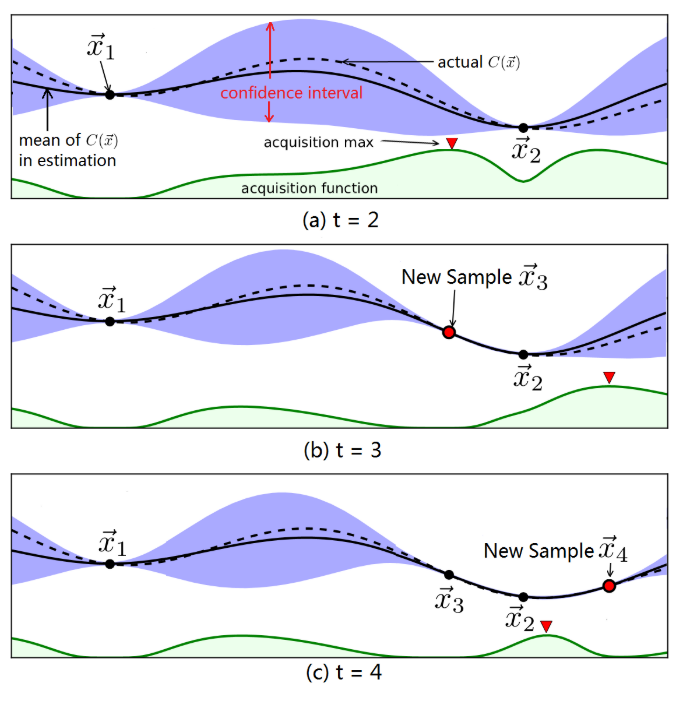
\includegraphics[scale=0.5]{Cherrypic}
  \caption{An example of BO's working process. Taken from Figure 5 in \cite{Alipourfard2017}}
  \label{fig:cherrypic}
\end{figure}

\paragraph{}
There are a number of possible prior functions, acquisition functions, and stopping conditions that can be used with BO, and the Cherrypick paper goes into detail on the reasoning behind which options are best for cloud configuration selection specifically\cite{Alipourfard2017}. There are some notable differences between their use-case and ours, however. CherryPick was specifically focused on batch jobs, where what is measured is simply a function of an instance type's cost and its time taken to perform a given job. Its acquisition function is specified to this purpose, minimizing costs but biased towards configurations which satisfy a soft performance constraint by successfully performing the batch job within a given time. In our case, our acquisition function must be more general, and we will therefore be relying on the user to ensure that whatever objective measure is returned by their Interpreter has already taken into account soft or hard performance constraints such as this.
\section{VM Docker Deployment}
Once the VMs themselves have been provisioned, the application must be deployed onto them. In the use case, we assume that the application being tested is available in the form of a Docker image, and that a single instance is provisioned on which to run that application. Docker offers a remote API with which one can direct the host machine to download an image and run a container based on it, as well as return the application's logs. In order to deploy an application onto a VM, that instance must first have Docker installed onto it and Docker directed to a public-facing port. The Deployer can then use the public facing IP of the provisioned machine along with user-provided security credentials to deploy the application. The Deployer can then obtain and return any and all logs the deployment produces for use by the interpreter.

\section{Search space encoding}
Whether using exact or closest match, it must be decided how to encode cloud configurations into a set of input variables. This problem is further complicated by the fact that constraints for certain inputs may depend on the values of others, as is often the case in cloud computing. Large memory amounts are often only available on VMs with more vCPUs, and some providers may offer available configurations others do not. Google Cloud Platform allows users to specify custom machine types, but even these do not allow any possible combination (for example, Memory constraints are tied to vCPU number, and vCPU number must be divisible by 2).

\paragraph{}
Despite these problems, there are at least clear patterns prevailing throughout leading cloud providers, such as separating instance types into categories equivalent to 'Compute-optimised', 'Memory-optimised', and 'Storage-optimized,' each with a set of machines with between 2 and 96 vCPUs. In lieu of a cross-provider service to match a given specification to a specific cloud instance type, these industry-standard categorisations can be used to encode the search space in a reasonable manner. Table \ref{tab:config-encode} shows an example of how we have used these patterns to encode 6 instance types into a set of 4 easily interpreted variables; Provider, vCPU number, memory, and machine category. A Selector could simply filter a dataset of this form to find the instance-types corresponding to a set of input variables. Users can extend or change the search space by providing their own datasets of the same format, with the same or different variables.

\begin{table}[!t]
\centering
\begin{tabular}{ |c||c|c|c|c|  }
 \hline
 Instance Type & Provider & Category & vCPU Number & Memory \\
 \hline
 n1-standard-2    & GCE  & General & 2 & 7.50 \\
 n1-standard-4    & GCE  & General & 4 & 15.00 \\
 n1-standard-8    & GCE  & General & 8 & 30.00 \\
 c5.large         & EC2  & CPU & 2 & 4.00 \\
 c5.xlarge    & EC2  & CPU & 4 & 8.00 \\
 c5.2xlarge    & EC2  & CPU & 8 & 16.00 \\
 \hline
\end{tabular}
\caption{A possible way of separating instance types into 4 descriptive variables. Providers were either the Google Compute Engine (GCE) or the Amazon Elastic Compute Cloud (EC2)}
\label{tab:config-encode}
\end{table}

\paragraph{}
In the end,  however, the important features and constraints for the search space will differ for each user, and it may be beneficial to run multiple experiments in different search spaces before settling on a final decision for an instance type. While we provide in our system an example of how to encode and select available cloud configurations for our Bayesian Optimization tool, that works well for cloud compute services, we think it best to ultimately leave it to the user to design and implement a Selector system that works well for their specific use-case.

\section{Objective Measure}
Our video transcoding benchmark returns the time taken to transcode a given video file, relative to a reference. We have assumed that our ultimate goal is to find the cloud configuration that will maximise the amount of video transcoding performed per unit cost. Though in a competitive business environment, even a small increase in transcoding speed may translate to large increases in customer uptake, our simple metric should effectively show how an benchmark score can be used with an instance price to generate an objective measure.

The vBench benchmark used, 'vod', returns a 0 if the video is not of a sufficient quality following transcoding. This effectively sets a hard constraint on performance, ensuring that no matter how cheap an instance is, it must achieve a certain level of performance to be selected.
We have noted that Cherrypick\cite{Alipourfard2017} instead incorporates constraints into the Bayesian Optimziation algorithm itself by including it within the acquisition function. This is not a generalized solution, however, and so we have instead incorporated performance constraints within the objective measurement itself.

\chapter{Implementation}
\section{General usage}
Our system\footnote{\url{https://github.com/briggsby/AutomatedBayesCloudSelection}} was implemented with a combination of Bash scripts and Python 3. Exhaustive search was performed using Bash scripts. The Searcher component was implemented using Spearmint\cite{Snoek2012}, an implementation of Bayesian Optimization in Python. Due to the design of Spearmint, the Searcher component was made to call a single core python script that would call user-specified functions that make up the Selector, Deployer, and Interpreter components. Several forms of these components were implemented, each as a set of Python functions. Extension of the solution by adding additional components is easily done by writing new Python functions that either directly perform the component's job or calls another tool to do so.

\paragraph{}
User-provided options, such as what Selector, Deployer, and Interpreter to use, as well as other user supplied variables, can be provided in the form of a JSON file that is read and loaded as a Python dictionary by the core script. This dictionary is passed as input to each component, which update it with any information needed by other components in the form of key-value pairs. At the end of any job, this dictionary object is saved in JSON format for later analysis and recovery of previous results.

\section{Searcher}
\subsection{Spearmint}
Spearmint is an implementation of Bayesian Optimization written in Python\cite{Snoek2012}. The user submits a single python script with an appropriate 'main' function which has its inputs optimized. Spearmint provides numerous settings for changing variables like the maximum number of concurrent jobs, acquisition function used, and sampling noise assumptions. However, the latest available implementation of Spearmint was found to be outdated and incompatible with the latest versions of various Python modules used in later steps. 

Because of this, for the sake of generalisability we first updated Spearmint to be compatible with Python 3 and newer versions of its dependencies such as Google Protocol Buffers. These edits mostly included changes to syntax inconsistent with new versions of its dependencies.

We also added in stopping condition arguments for the 'chooser' modules. These modules are responsible for performing the acquisition function to determine the next samples to take. Our added arguments allow users to specify stopping conditions for the search based on expected improvement (EI) thresholds and minimum number of samples. This further automates the search, as beforehand the user was required to manually stop the search.

This implementation of spearmint has been made publicly available\footnote{https://github.com/briggsby/spearmint3}. 

\subsection{Search space encoding}
Spearmint uses their own protocol buffers to allow users to specify the available input variables. Each variable must be typed as either an integer (INT), floating-point number (FLOAT), or categorical variable (ENUM). For the first two, minimum and maximum limits must be set, while for categorical variables each available option must be specified. For all variables, a 'size' is specified, and each variable is passed to the function as a Numpy\cite{Klein2014} array with a number of elements equal to its 'size.' Each of these elements is optimized individually.

This format of encoding variables sets some limitations. Constraints for numeric values are limited to minimum or maximums. For an example of where this is insufficient, vCPU numbers for custom instance types on Google Compute Engine are limited to even numbers. While there are methods to get around this, such as encoding vCPU number as an integer which is then multiplied by 2 by the submitted script, in some cases it can lead to repeated job failures as impossible inputs are repeatedly attempted.

To get around this problem, the vCPU number was specified instead as a categorical variable, and other than that the encoding is identical to that described in the Design section, except without using the Memory variable:
\begin{enumerate}
\item vCPU number was encoded as a categorical variable of size 1 with options '2', '4', and '8.' 
\item Provider was encoded as a categorical variable of size 1 with options 'aws' and 'google', corresponding to Amazon EC2 and Google Compute Engine respectively.
\item Category was encoded as a categorical variable of size 1 with options 'General,' 'Memory,' and 'CPU.'
\end{enumerate}
\section{Driver}
The Driver script is a single python file called by Spearmint, and as such must take as parameters only the Job ID (a number used to identify jobs within a single spearmint experiment) and input variables as a multidimensional array.\\
Our Driver immediately reads a local configuration file in JSON format and loads it as a Python dictionary. This configuration dictionary stores relevant information in a set of key-value pairs, such as the user-specified Selector, Deployment, and Interpreter components, and other variables such as the Docker image address and container runtime commands. Both the keys and values are specified within the files, to make sure that the implementation is extensible to any later added components. This configuration dictionary is updated with the input variables submitted with that job, and passed as a parameter to the functions specified as the framework components. It is later saved to a local JSON file at the end of the job for record-keeping and debugging purposes. \\
The Driver script responds with a single value, the objective measure to be minimized by the Bayesian Optimization process.
\section{Selector}
\subsection{Exact Match}
A CSV file was created with the following variables for the instance types used in our evaluation:

\begin{itemize}
\item API Name - Name of instance type used in that provider's APIs (string)
\item Provider - Cloud provider offering the instance type (string)
\item CPU - Number of vCPUs (float)
\item Memory - Amount of memory in GB (float)
\item Category - Category of machine type, such as Compute or Memory optimized, in a consistent form between providers (string) 	
\item Price - Hourly cost of the machine for an On-demand Linux image (float)
\end{itemize}

The Selector loads this dataset as a Pandas dataframe, iterates through the input variables provided, and filters the dataframe accordingly. The configuration dictionary is then updated with the API name and hourly cost for the cheapest option remaining, and returned by the function. If no configuration is left in the filtered dataframe, these values are instead set to a Null value, to indicate that no configuration exists. This script is compatible with any set of input variables specified, provided that the dataset has a column corresponding to each of those variables.

\section{Deployer}
\subsection{VM Provisioner}
The first stage of any tested deployment was to first provision the necessary VMs from their cloud provider. To do this, we implemented the IaC tool Terraform, using a Python library python-terraform\footnote{https://github.com/beelit94/python-terraform}. 
\subsubsection{Terraform}
Terraform operates by applying 'plans' based on Terraform configuration files and variables provided either during the applying step or in separate 'tfvars' files. For each provider, a separate folder was created with a corresponding Terraform configuration file. The configuration files would, when applied using Terraform, provision a number of machines of a given type from the corresponding provider, and set up a publicly accessible Docker host on each machine. This is done by first setting up a security rule exposing a specific port, later used by Docker. The machine of the given type is then provisioned, and using SSH Docker is installed, using either the Amazon Linux Extra library\footnote{\url{https://docs.aws.amazon.com/AWSEC2/latest/UserGuide/amazon-linux-ami-basics.html\#extras-library}} for AWS machines, or using a downloaded script from \url{https://get.docker.com} for Google Cloud Platform machines. In either case, configuration files are uploaded and the Docker service restarted to expose it to an external port for remote access in later steps.

\paragraph{}
The number and type of machines, specified by the input variables, are input when the Terraform plan is applied based on the job being run. Other important variables, such as credentials file locations, are placed by the user beforehand in a single 'tfvars' file in the same folder as our driving Python script. This file is shared between all Terraform plans, regardless of provider. The Terraform plan outputs a timestamp, the configuration details, and the public IP. These outputs are placed in the configuration dictionary for use by later Deployment steps.

\paragraph{}
When Terraform is directed to a folder, it automatically applies plans from all Terraform files located in that folder. It was important that we could run multiple Terraform plans at once, but using a separate configuration setup for every job would lead to extremely large disk usage and overhead, as Terraform must download necessary modules into the local folder for initilization before applying plans. Because of this, each deployment job was instead made to use the same plan, but a different 'local back-end,' storing the state files in a separate folder. Output values are only taken from the standard output returned when the configuration plan is first applied, as attempting to get the outputs later can lead to returning outputs from different back-ends when separate deployments attempt to obtain this information at the same time.


\subsection{Docker deployer}
Once the provisioned VM is finished its set-up as a Docker host, control is returned to the Deployer, which then connects to the Docker host through its public IP. This is done using the Python Docker library. The docker image specified in the configuration dictionary is then deployed on the connected client, and any parameters stored in the configuration dictionary under \textit{docker\_params} is passed as well, allowing additional entrypoint commands or hosted volumes to be specified. The Deployer attaches to the container until its runtime is completed, and then places the container's logs in the configuration dictionary for use by the Interpreter.

\paragraph{}
No Docker image was available for vBench at the time of writing, and so we created an image containing vBench that installs all its necessary dependencies and contains all video files used for reference scores. This is available on a public DockerHub repository at \textit{briggsby/vbench:ubuntu}. It takes command-line arguments in the form "\textless type\textgreater \ [filter]". 'type' specifies the type of benchmark to run: One of 'upload', 'live', 'vod', 'popular', or 'platform'. 'filter', if present, is a string that tells vBench to run the benchmark only on files whose filenames match that string, using asterisks as wildcards.

\subsubsection{Simulated vBench}
Also included is a Deployer component that uses results taken from our evaluation to simulate vBench deployments (for the 'house' video file using the 'vod' benchmark) on the tested instance types. This can be useful when debugging to avoid search costs and drastically reduce the search time by preventing the system from having to provision and set up virtual machines. The simulated results come from a normal distribution with the same mean and standard deviation as the results taken during evaluation.

\subsubsection{Cloudsuite}
Our described implementation assumes a single instance and a single Docker image, but this is not always the case. Included in our implementation is a deployment option for deploying the Cloudsuite3\cite{Palit2016} media-streaming server benchmark. This was originally planned to be used as the evaluated benchmark, but was found to be far too variable and showed no clear relationships with any input variables. \\
The Cloudsuite3 media-streaming benchmark requires multiple Docker containers to be set up on the same device on the same Docker network. The Deployer for it first deploys an image containing a dataset used by the benchmark server, followed by deploying the benchmark server itself and telling it the dataset location on the network. \\
The third part of the Cloudsuite3 media-streaming benchmark is an image that simulates multiple clients attempting to utilize the media streaming server at a time. However, the maximum number of clients used by the provided image was far too low in all cases. Our Deployer instead builds a new image, based on the original Cloudsuite3 image, that allows command-line arguments to specify maximum number of sessions and number of clients when deployed. The files necessary for this are included with our implementation.\\
Once again, this Docker container is left to run until it has finished, and the logs are then saved to the configuration dictionary for interpretation.
 
\subsection{Ping servers}
In some cases, internal performance measures from within an application may not be best suited to benchmark its performance, or it may simply be more convenient not to develop a whole new application that can self-report performance when an alternative is to use information from an application's connecting clients. 
In these cases, a separate server can be used to simulate network requests to a tested application. As this is a dramatically different approach to application performance testing compared to our Docker Deployment method described above, we wanted to include its implementation to highlight the flexibility of our framework.
For the Ping server Deployer, a separate Kubernetes cluster must be provisioned beforehand, and its details and credential file locations written into the configuration file. This Kubernetes cluster is used as a 'ping cluster,' and logs are taken from it rather than from the application itself. The application is deployed on the specified cloud configuration as normal, but no logs are taken from it. Instead, a pinging Docker image is deployed onto the ping cluster and its logs taken when its runtime has completed. These logs are interpreted instead of the application's. In our example implementation, the application itself is a webserver than simply calculates the highest prime number below a number requested by a client. The client Docker image deployed on the ping server repeatedly uses \textit{curl}, directed to the public IP of the application using a random number request from a normal distribution, and returns the time taken to receive the response for each request along with the number requested.  
\subsection{Instance removal and Interruption handling}
Whatever Deployer is used, once the logs have been taken from a sample deployment the instances provisioned must be terminated so as not to continue accruing costs or use up cloud provider quotas. Terraform includes a 'destroy' command which uses the state files and Terraform plans to go through and remove any settings and terminate any virtual machines or services set up by that plan.
When the plan is first applied, a handler is set up to catch keyboard interruption signals and immediately trigger the Terraform destroy process, to ensure that even if an experiment or individual job is stopped early, cloud services are still immediately dismantled. 
\section{Interpreter}
As described previously, log interpreters are highly specific to any given use-case. They use the information extracted from the application logs by the Deployer, along with the price of the cloud configuration supplied by the Selector, to calculate the objective measure to be optimized by the Searcher. This objective measure is saved to the configuration dictionary as the final value to be returned by the core Driver file. Here we describe the three Interpreter components implemented.
\subsection{vBench}
The vBench interpreter extracts from the first video file transcoded the final vBench score provided and divides its negative by the price of the cloud configuration tested. The value's sign is reversed to ensure that the value is maximised by the optimization algorithm rather than minimized, as a higher score reflects a higher performance. If a performance threshold is met, the score reports the time taken to transcode the video file relative to a reference. If the performance threshold is not met, the score is 0. Once divided by the price, it gives the objective measure as the rate of video transcoding per hourly cost of the instance in US dollars. 
\subsection{Sysbench}
Sysbench is a commonly-used lightweight micro-benchmarking tool. In our case, we used it to measure how many times the instance can calculate the prime numbers up to 5000 in 10 seconds. The Interpreter uses regular expressions to extract the reported 'events per seconds.' Once again, this score has its sign reversed and is divided by the price of the configuration.
\subsection{Cloudsuite}
The Cloudsuite3 media-streaming server benchmark Interpreter uses regular expressions to extract from the application logs the maximum number of sessions for which the benchmark succeeded. If the maximum number attempted was too low for the benchmark to ever fail, it instead uses this maximum number attempted. Once again, this extracted value has its sign reversed and is divided by the price of the configuration.
\chapter{Evaluation}
\section{Evaluation Approach}
To demonstrate the effectiveness of our system and associated framework, we wanted to show both that it could take any individual sample within the implemented search space without problem, and also that it could carry out an entire optimization process. 
\paragraph{}
For the former, to show the system's ability to take individual samples, we wanted to show that the individual components for Selecting, Deploying, and Interpreting logs of a single application deployment job effectively carried out their purpose. To do this, we performed an Exhaustive search of the implemented search space for our vBench benchmark, taking 20 samples of each available configuration.\\
For the latter, to show the framework and system's ability to correctly select the optimal cloud configuration for a given application, we attempted to replicate CherryPick's\cite{Alipourfard2017} process and perform our Bayesian Optimization use-case, to ensure that it was effective at selecting the optimal configuration. The optimal configuration itself could be determined using the results from the exhaustive search. We will show how this Bayesian search varies according to different options used, such as the number of concurrent jobs allowed or the number of providers included in the search.\\
To show the flexibility of the Framework, we also wanted to test out a Bayesian Optimization search for the Ping server Deployer described in our Implementation chapter. This Deployer is impossible to run concurrently without multiple ping clusters, and so performing Exhaustive search would be extremely time-consuming and was not performed. \\
Finally, through this process we will generate many results regarding vBench scores across different machines, and how the Bayesian optimization process is affected by factors such as the number of concurrent jobs allowed and the size of the search space. We will present, statistically analyse, and discuss these findings.

\paragraph{}
Where not otherwise specified, statistical results are quoting P-values returned from a Tukey's Honest Significant Differences test to correct for multiple comparisons. This test looks at the probability that the means of two groups are significantly different, correcting for multiple comparisons, assuming that observations are independent and that groups are normally distributed with similar within-group variance. While, using raw vBench scores as an example, several instance types returned a significant result from the Shapiro-Wilk normality test, this test is very powerful and often returns low P-values for samples that can approximate a normal distribution. In addition, many  instance groups did not give significant results to the normality test, with several extremely high P-values above .50 returned. Variances were extremely low and consistent across groups. This, combined with a visual examination of the distributions of our results, such as those shown in figure \ref{fig:vbench-dists}, as well as the clear patterns observed from our graphical representations of our results, make us confident in the validity of our findings from the Tukey's tests.

\paragraph{}
Analysis was performed in RStudio\cite{RCoreTeam2018,RStudioTeam2016}, and full logs as well and scripts used for analysis are available on the project's Github repository. Generally, P-values were reported while effect sizes were not, as the effect sizes are extremely dependent on the test run and performance measure used and likely to be of no concern, if not outright misleading, when compared with other results.

\subsection{vBench}
Our objective function, a deployment of the vBench benchmark, measured an instance type's relative rate of transcoding of a single 5 second 1920x1080 video file, returning a score of 0 if the quality was below a given threshold, divided by the hourly price of that instance. This is the score given using the 'vod' benchmark type in vBench.\\
Effectively, we maximised the rate of transcoding a unit of video length at a sufficient quality per hourly cost. We had hoped to show that incorporating the soft constraint on video quality within the value returned by the Interpreter, rather than within the acquisition function as was done in Cherrypick, did not hinder the optimization process, however no instance type tested failed to achieve the threshold video quality in any sample.

\subsection{Ping server}
Having performed evaluation on our system for a deployment of a simple docker container with our vBench application, analogous to running a single batch job or benchmark and interpreting the results, we then wanted to evaluate the same technique applied to an web-based application. This application type may be better evaluated through its responses to a client, rather than from measuring its performance internally. For this a single 5-node Kubernetes cluster was set up for the purpose of sending repeated requests to the evaluated deployment, as described for the 'Ping server' deployer and interpreter. The mean response time for requests of a normally distributed load was divided by the hourly cost of the instance to give maximised value. 

\subsection{Search Space}
For choosing the boundaries of the search space, we decided to reduce costs by using only machines ranging from 2 vCPUs to 8 vCPUs. This was also convenient as to use more powerful machines would have required requesting additional raised quotas from the providers used, and so would be less easily replicable by others wishing to repeat our evaluation. As we wanted to show that the system worked with multiple providers, and were were ensuring our input variables matched exactly to an available instance type, we could not rely on Google Cloud Platform's custom machine types. Table \ref{tab:instance-types} show which machine types corresponded to input variables, as described in our Implementation chapter. 

\begin{table}[!ht]
\centering
\begin{tabular}{ |c||c|c|  }
 \hline
 & \multicolumn{2}{|c|}{Provider} \\
 \hline
 Machine Category & Amazon EC2 & Google Compute Engine \\
 \hline
 General& n1-standard & m5\\
 Memory & n1-highmem  & r5\\
 CPU    & n1-highcpu  & c5\\
 \hline
\end{tabular}
\caption{Machine types corresponding to different instance categories for the two providers}
\label{tab:instance-types}
\end{table}

The 18 machine types decided upon (3 vCPU numbers for 3 machine categories for the 2 providers) were stored in a single CSV dataset for use with the instance Selector. A vBench Deployer was used which utilized Terraform to provision a single instance of the given machine type, on which the remote docker API was used to deploy and collect logs from an docker image containing vBench. An Interpreter then isolated the vBench score from these logs, and divided it by the hourly cost of that machine type to return the final value.

\section{Framework and System Evaluation}
Looking back at our first chapter, we are confident that the evaluation below shows that we have succeeded at all aims and objectives previously presented. The Bayesian Optimization results show that the system, based on our framework, was capable of fully automating the process of selecting an optimal cloud configuration for a given application. We have shown that this is not application or provider specific, performing the process across multiple providers (Amazon EC2, Google Compute Engine) and utilizating multiple cloud services (Kubernetes clusters, single VM instances), to test it across two very different applications (Web serving application, video transcoding benchmark). This process accounted for the recorded variation within instance types for application performance, and produced accurate predictions. Using our system, we successfully sampled application performance and cost-effectiveness across every available configuration within our search space, performing an exhaustive search. Using this complete analysis of the potential configuration options and their relative performance, we were able to measure the success of our Bayesian Optimization system with various search options.

\paragraph{}

For the vBench benchmark application, in the best experiment setup found (Multiple providers, 2 concurrent jobs) our Bayesian Optimization experiment correctly identified the optimal instance type in 18 out of 20 repetitions. The mean value returned with this search setup was at the 98th percentile of possible scores from the available search space.

From the samples taken during 10 repetitions of the ping server experiment, it seemed that there were no significant difference between the two best performing configurations of c5.large and m5.large instance types ($\Delta \bar{x}=0.0001, P \approx 1.000$). The predictions correctly converged upon one of these instance types in all 20 repetitions of the Bayesian optimization search.



\section{Results Analysis}
\subsection{Exhaustive search}
\subsubsection{Results}
\begin{sidewaysfigure}
  \centering
   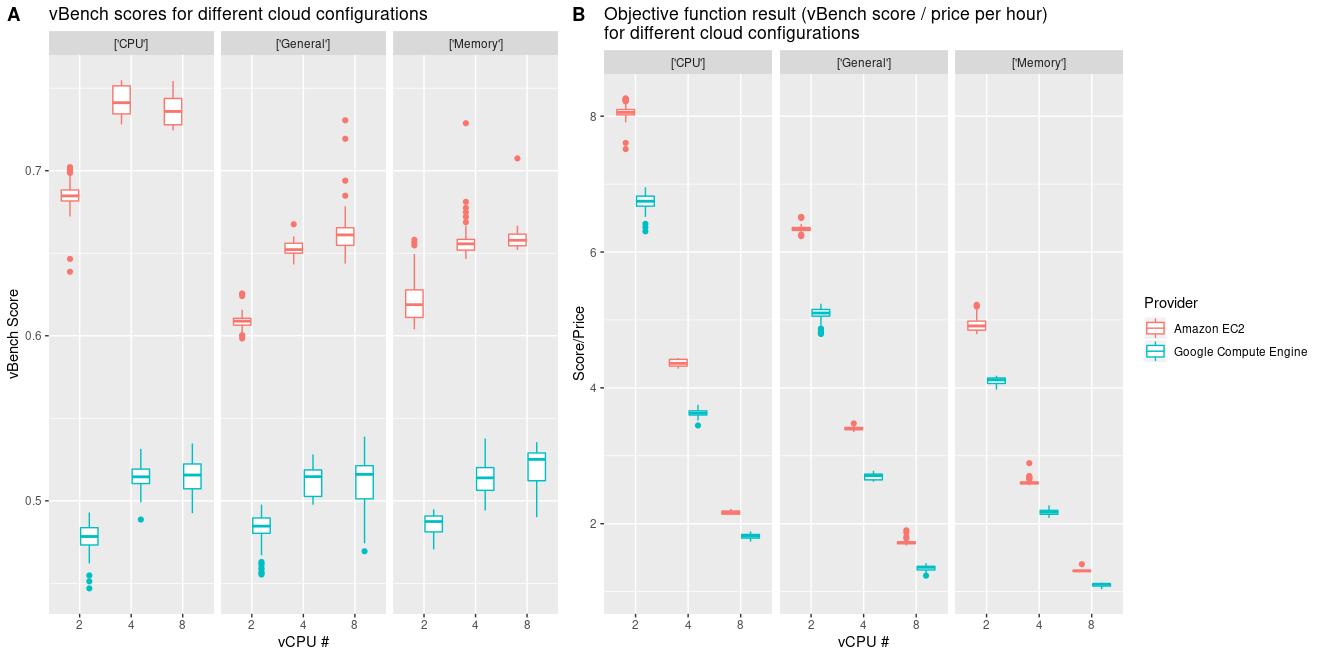
\includegraphics[scale=0.6]{exh_search}
   \caption{Boxplots showing the distribution of vBench scores and objective measure values (both plotted on y-axis, different scales) across different machines, differentiated by cloud provider (colour), instance category (columns), and number of vCPUs (x axis). vBench benchmark was run using the 'vod' benchmark type and the provided 5 second 'house\_ 1920x1080\_ 30.mkv' video file reference score.}
  \label{fig:exh-search}
\end{sidewaysfigure}

The results of the exhaustive search are shown in figures \ref{fig:exh-search} while the distribution of scores for each instance type are shown in frequency polygon form in figure \ref{fig:vbench-dists}.

\begin{figure}[!ht]
  \centering
   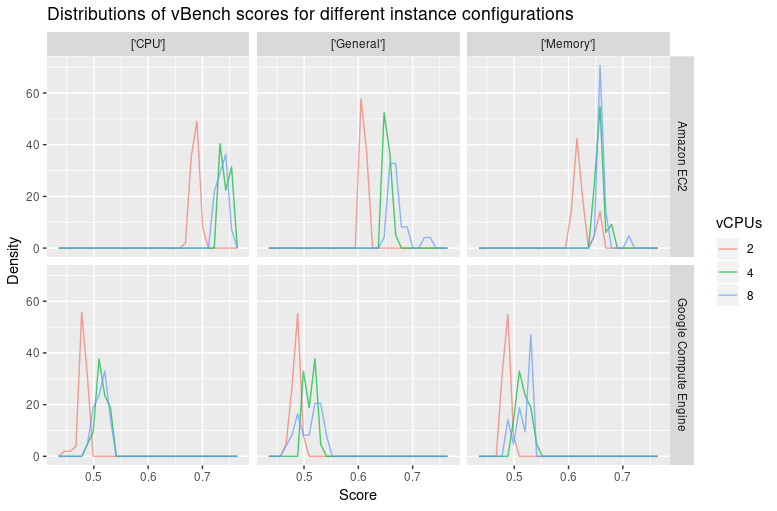
\includegraphics[scale=0.7]{vbench_dists}
   \caption{Distribution of vBench scores in frequency polygons. Higher peaks represent more common scores. The columns separate the instance category, rows separate the cloud providers, while color distinguishes the number of vCPUs available in that instance. vBench benchmark was run using the 'vod' benchmark type and the provided 5 second 'house\_ 1920x1080\_ 30.mkv' video file reference score.}
  \label{fig:vbench-dists}
\end{figure}


Relative standard deviations for all scores measured were very low, the highest being $\pm 3.23\%$ for the n1-standard-8 instance type. No relationship with this variance was found for any of the three search variables.

The raw scores (time taken to transcode relative to the reference) show clear overlap between many possible configurations. In general they show a significant difference between 2 vCPUs and either 4 ($P < .001$) or 8 ($P < .001$) vCPUs, and between 4 and 8 vCPUs ($P < .001$), where the score increases with vCPU number, when accounting for differences between provider and machine category. However, the effect size is dramatically diminished between the 4 to 8 categories ($\Delta \bar{x} = 0.0116$) compared to that between the 2 to 4 categories ($\Delta \bar{x} = 0.0526$).

However, once the scores are divided by that machine's hourly costs, to give the objective measure value, there is much less overlap. If one is purely interested in getting the most video transcoding for a given cost, a clear optimal configuration can be seen in the c5.large machine type. The c5.large machine was significantly better than the next best option, the n1-highcpu-2 ($P < .001$), as well as all other options (All $P < 0.001$). Amazon EC2's  machine types consistently outperformed Google Compute Engine's equivalents of the same category and vCPU number at both raw score (Anova, $F = 32111.456, P < .001$) and value for money (Anova, $F = 22710.7, P < .001$). While provider was the most important determining factor as to whether a cloud configuration gave a higher raw score than others, it was the least important determining factor as to whether a cloud configuration gave a higher objective measure value. For example, the n1-highcpu-2 still gave significantly better values than the m5.large ($P < .001$), or the c5.xlarge ($P < .001$) making it the second most cost-efficient option. 


\subsubsection{Discussion}
Our results concerning CPU performance variability within instance types are consistent with a recent study \cite{Scheuner2018} confirming that the newer instance generations are considerably more stable than previous ones \cite{Leitner2014}, drastically reducing performance variability. In many cases, we could likely have assumed noiseless sampling for our Bayesian Optimization searches and received identical results. Our sampling noise values, referring to the original standard deviation for objective measure without division by the mean, was consistent enough between instance types that no log transformation was necessary for the Bayesian Optimization performed, as was done in the Cherrypick measure to ensure sampling noise was consistent and additive even when reported as a value relative to the mean\cite{Alipourfard2017}.

We observed very notable diminishing returns in the increase in performance for increasing vCPU number above 4 vCPUs. Despite the cost of instance types continuing to rise proportional to the number of vCPUs, there was an approximately 5-fold reduction in score gain between 4 and 8 vCPUs compared to 2 and 4 vCPUs. This suggests that the video transcoding process measured by our benchmark has diminishing returns past 4 vCPUs, possibly due to an inability to parallelize in such a way to utilize more cores.

Our results also showed that Amazon EC2 instances drastically outperformed the Google Compute Engine instances tested at video transcoding operations, regardless of other variables. Even the best-performing Compute Engine instance returned a score much lower than the worst-performing EC2 instance ($P < .001$). Google in general used older Intel Processor models in their machine, which may account for this disparity in performance.

Once cost-effectiveness was examined instead of raw scores however, cloud provider instead became the least important variable. However, when the other variables of instance category and vCPU number were the same, AWS instances still outperformed their Google Compute Engine equivalents.

Our results clearly show that, for maximising the rate of video transcoding for our tested video file per dollar spent, the Amazon EC2 instance type c5.large was the most efficient instance in our tested search space. 
\subsection{Bayesian Optimization}
\subsubsection{Results}
With the exhaustive search complete, we then used a Spearmint based searcher to perform a Bayesian Optimization search, assuming low noise (-1 to 1) and using the same stopping conditions as used by default in the Cherrypick paper \cite{Alipourfard2017}, namely when the Expected improvement (EI) is less than 10\%, and at least 6 samples have been taken. We were able to successfully run this experiment with both multiple and single providers, as well as with between 1 and 3 multiple concurrent jobs.

\begin{figure}
  \caption{Optimal configurations suggested after convergence for Bayesian Optimization searches. Bayesian Optimization attempted to maximize the vBench 'vod' score divided by the configuration price. Prior function used was a Gaussian process, with Expected Improvement used as an Acquisition function. Searches were stopped at N $>$ 6 and EI $<$ 10\%, and the shown configuration was the instance with the best returned value.}
  \label{fig:bo-results}
  \centering
  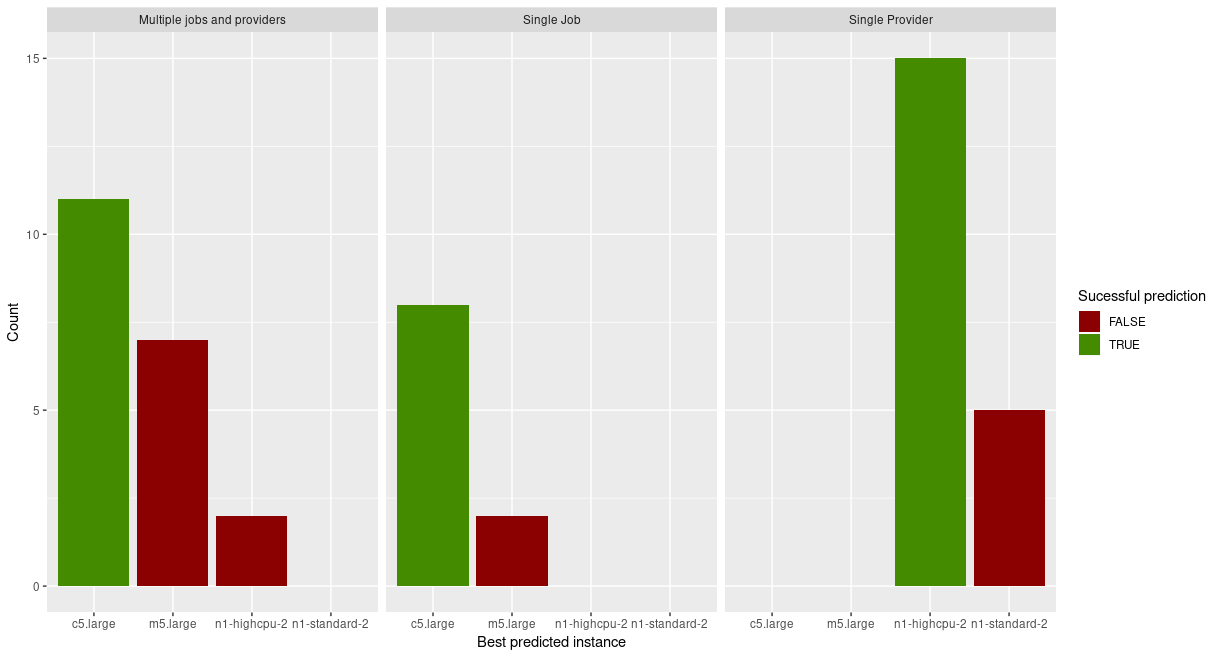
\includegraphics[scale=0.5]{bo_results}
\end{figure}

The results from these experiments are shown in figure \ref{fig:bo-results}. When testing instances from only a single provider, and running only a single concurrent job at any time, we were able to replicate the findings of the Cherrypick paper \cite{Alipourfard2017}. In 17 of 20 experiments, Bayesian Optimization was able to reach the same conclusions as Exhaustive search in only 6-12 samples, with a mean performance that was approximately 96.9\% of that from the optimal possible configuration. 

Even when the number of providers was increased from 1 to 2, with only a single concurrent job running, we were also able to replicate the previous results. The correct optimal instance was predicted in 18 out of 20 evaluations, in only 6-11 samples (97.9\% relative mean performance). For our evaluation, despite doubling the search space, Bayesian Optimization was no less effective.  It may be interesting to note, however, that the incorrectly predicted instance in both failed cases for multiple providers was not the second but third best choice, coming from the same provider rather than the other.  Figure \ref{fig:bo-boxplots} shows box-plots for the optimal values, time taken, and search cost for all Bayesian Optimization experiments run. It can be seen from this that there was no clear negative effect on the relative effectiveness of the search between single or multiple providers ($ P = .999 $). There was similarly no clear increase in time taken or search cost. Examples of the job paths taken during both one of these successful searches, as well as an unsuccessful one, are shown in figure \ref{fig:paths}-C \& \ref{fig:paths}-D. 

Within figure \ref{fig:bo-boxplots}, the optimal values are presented as a proportion of the best possible result, estimated from the mean result of all jobs run on the instance in that search space with the highest mean value. Search time was calculated from the difference in time between the last and first completed job. This time does not include initial setup or time taken to terminate any unfinished jobs once the search was stopped. Relative search cost was calculated by summing the hourly cost of the instances samples, including repetitions. This assumes that either every job took the same amount of time regardless of instance, or that the applications were short enough ($<$1 minute) to accrue only the minimum possible cost for provisioning each instance type. Even on the slowest instance type tested, our vBench benchmark completed in approximately ~35s, so we are confident that this second assumption holds.

\begin{figure}
  \caption{Values, search costs and search times for different Bayesian Optimization searches. A single large outlier was removed from the search time graph (4000s) from Single provider, 3 concurrent jobs, for legibility. In single provider tests, only Google compute Engine was involved. 'Best values' shows the values the search returned as a proportion of the optimal possible value the search could attain, calculated from the mean value available from jobs run on the best instance in the search space. Search time calculated by measuring the time between the first and last sample taken. Search cost taken by multiplying each job by that instance's hourly price and summing these values. 'Ping test' test type used latency of responses to a web-server, while other tests used a vBench 'vod' benchmark. Searches were stopped at N $>$ 6 and EI $<$ 10\%}
  \label{fig:bo-boxplots}
  \centering
  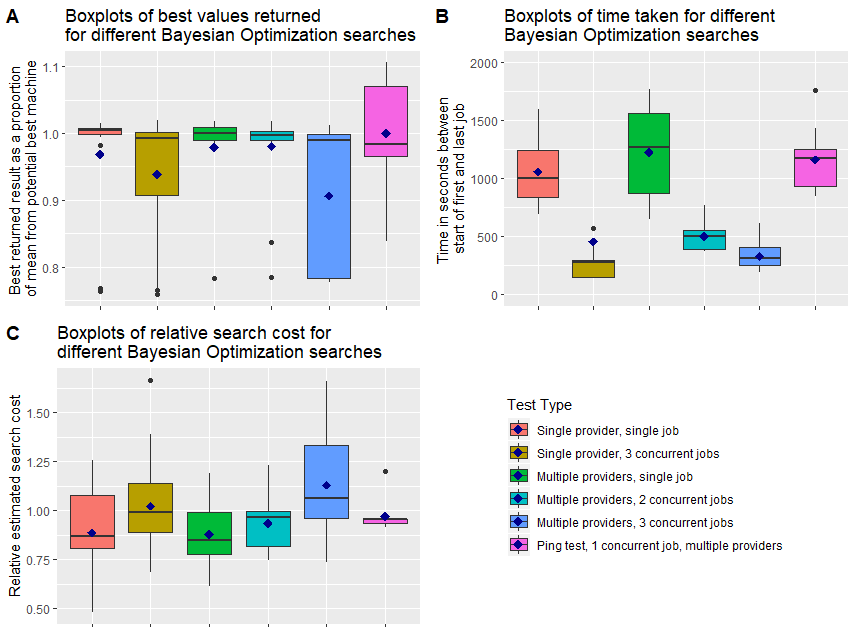
\includegraphics[scale=0.7]{bo_boxplots}
\end{figure}
\begin{figure}
	\centering
	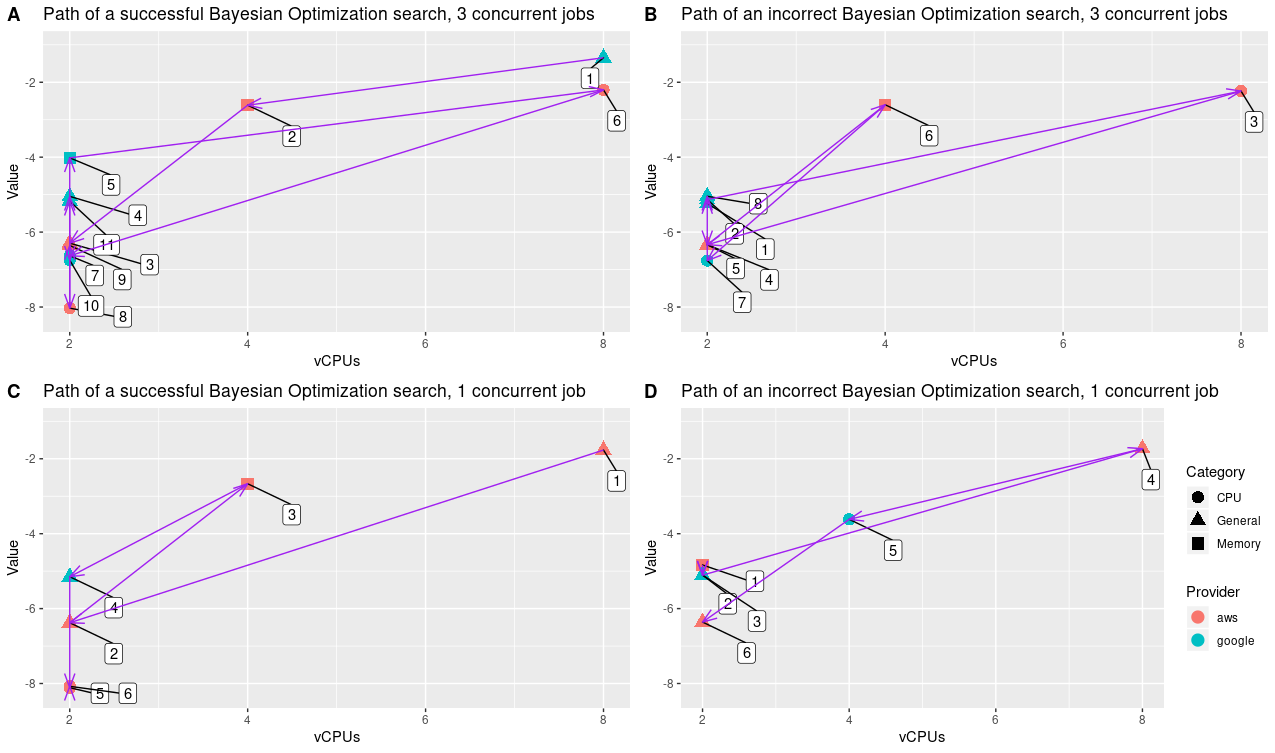
\includegraphics[scale=0.4]{paths}
	\caption{Paths of example Bayesian Optimization jobs to optimize a vBench 'vod' score. Numbers and arrows show the progression of paths, with each point representing a different cloud configuration sample. The y-axis shows the objective measure value returned by the sample. Colour shows cloud provider, either Amazon EC2 (aws) or Google compute engine (google).}
	\label{fig:paths}
\end{figure}

We then looked at the changes to the search results when multiple concurrent searches were allowed. By allowing 2 concurrent jobs to be run at any one time, the time taken for the search was reduced to less than half that of before ($P < .001$). Along with this  dramatic reduction in time taken, there was no rise in search cost ($P = .95$). The number of completed jobs performed was still between 6 and 10 in all experiments. Even more impressive, there was also no loss in the optimal value returned ($P \approx 1.00 $), with it still choosing the correct instance in 18 out of 20 repetitions, with a mean relative value of 98.1\%.

However, increasing the number of concurrent jobs higher, to 3, caused a dramatic reduction in effectiveness. For multiple providers, the experiment returned the optimal instance in only 11 out of 20 repetitions (mean relative value of 90.1\%). The probability of returning a sub-optimal value may increase compared to 1 concurrent job ($ P = .09$) and 2 concurrent jobs ($P = .08$). The increased maximum allowed job concurrency also increased the search cost compared to 2 concurrent jobs ($P = .03$), and did not lead to any significant further decrease in search time ($P = .81$). To ensure this held true even in a reduced search space, the experiment was repeated with 3 concurrent jobs but only a single provider, to similar results.

\subsubsection{Discussion}
For a single provider and a single maximum concurrent job, and stopping criteria of an expected improvement less than 10\% with at least 6 jobs completed, similar search conditions to that of the CherryPick paper\cite{Alipourfard2017}, we were able to replicate their results for our video transcoding benchmark. Bayesian Optimization, in few samples, was able to accurately identify the optimal configuration, confirmed by our Exhaustive search, in 85\% of our experiment's repetitions. Even when a less than optimal instance was returned by the search, performance for these instances was still high enough to give a mean returned value in the 95th percentile for performance. Our modifications to Spearmint mean that in our system's provided implementation the stopping conditions can be easily specified at runtime, to allow the user to tighten or loosen these stopping conditions as their use-case requires.

We expanded on previous findings by testing the same search when expanded to multiple providers, and with multiple allowed concurrent jobs.

Bayesian optimization was shown to be very resilient to the increased search space introduced from adding a cloud provider, with no loss of effectiveness or efficiency. This was likely because the large and consistent performance difference between Amazon EC2 instances and Google Compute Engine instances meant that the Searcher was very quickly confident that the 'provider' variable had been optimized throughout the search space. A difference in search effectiveness may have been seen if the performance difference between providers was small rather than large, or if the relationship was more complex and dependent on other variables.

When 2 concurrent jobs were allowed, the effectiveness and cost-efficiency of the search was unaffected, but the time taken to perform it was dramatically reduced. Past 2 concurrent jobs, allowing further concurrency reduced the search's effectiveness without any further benefit. This suggests that it is beneficial for users to allow 2 concurrent jobs, but not to allow any more, at least for our example use-case. 
\chapter{Related \& Future work and Conclusion}
\section{Related work}
We have successfully replicated the findings of the CherryPick\cite{Alipourfard2017} paper, confirming the effectiveness of Bayesian Optimization. We expanded on their findings to show that while concurrent jobs can reduce search time without a loss of accuracy, too many concurrent jobs can reduce accuracy without further reducing search time.

In our literature review, we examined multiple solutions for cloud configuration selection, such as Ernest\cite{Venkataraman2016} or PARIS\cite{Yadwadkar2017}. We have taken care to ensure that our framework does not preclude these solutions, and their designs can be incorporated into it. Even PARIS, with its markedly different approach to configuration selection compared to other solutions, could be replicated in our framework by developing a Searcher that first uses the other components to run the application on user-defined reference VMs, followed by searching through available configurations using a Deployer that, rather than running new deployments, runs a random forest model based on these results and previous benchmark scores. 

\section{Future work}
As stated throughout the design and implementation of our framework and system, there are numerous avenues for extension of our system through the development of different component modules. In particular, we present three suggestions for further research:

\paragraph{GPU Instances:} Our results do not tackle set up of drivers necessary to make use of GPU instances. GPU instances have been shown to be well suited for live-streaming media servers\cite{Lottarini2018}. A Deployer would have to be developed that can install necessary drivers and ensure an application can make use of a VM's available GPU.
\paragraph{Serverless services:} Serverless services are particularly opaque as to their performance. Once APIs are available for Terraform or other IaC tools for services such as Google Cloud Run our framework could illuminate performance differences between available serverless providers.
\paragraph{Expanded search space:} In general, our study was limited in its search space. Our provided Selector dataset spans the instances from Google Compute Engine and Amazon EC2 that do not require additional requested quotas. Expanding this to larger machines or to other providers, such as Microsoft Azure, is a straightforward way to improve its scope. 
\section{Summary}
All objectives set out in the Introduction were successfully achieved, producing a framework for automated selection of a cloud configuration, generalized for any application or search space of cloud services. A system was produced, with a functional publicly available instantiation, that was effective in predicting optimal compute instance types for a video transcoding benchmark, but is also applicable for any application that can be contained in a single Docker image to be deployed on a single instance type. The system is modular by design, and is easily extensible for new use-cases or cloud services, and with extensions would be capable of replicating many previous solutions published for cloud selection. The use-case was chosen and the system designed in a manner mindful of the time-constraints the project presented, but a successful solution was produced that will greatly benefit from future development and contributions.
\newpage
\bibliographystyle{ieeetr}
\bibliography{Dissertation}
\newpage
\end{document}
